\documentclass[main.tex]{subfiles}

\begin{document}
\subsubsection{VGA-motor}
\begin{SCfigure}
    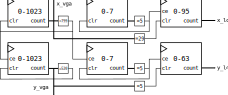
\includegraphics[width=0.85\textwidth]{vga.eps}
    \label{fig:vga}
    \caption{Räknarna inom VGA-motorn.}
\end{SCfigure}
VGA-motorns primära uppgift är att visa upp miniräknarens bildminne på
VGA-skärmen. VGA motorn räknar igenom varje pixel på skärmen rad för rad och
skickar dess pixelfärg. Två räknare används, en för raden (\mono{y\_vga}) och
en för kolumnen (\mono{x\_vga}). Utifrån räknarnas nuvarande värde bestäms även
hsync och vsync-signaler. Mer information om hur VGA-standarden fungerar samt
exakta timings kan hittas i Nexys3-manualen.\cite{nexys3}

Eftersom VGA-skärmen är $640\times480$ och miniräknarens LCD-skärm är
$96\times64$ kan varje pixel som mest var $6\times6$ pixlar för att hela
skärmen ska rymma. Om pixelbredden var en potens av två skulle det gå avgöra
vilken pixel från bildminnet som skulle ritas utifrån de högre bitarna i
\mono{x\_vga} och \mono{y\_vga}.

För att visa upp en bild på skärmen måste data skickas till varje pixel om
vilken färg den ska ha. VGA-motorns ansvar är att räkna igenom alla pixlar på
skärmen och tilldela dem data i form av en 8-bit RGB färg. I TI83:an kan pixlar
endast vara av och på. Därför, för att representera dessa, används bara två
färger i monitorn. Svart som ritas för pixlar som är på och en blågrön nyans,
som påminner om origanlskärmens färg, som ritas för pixlar som är av.

Bildskärmens upplösning är 640x480 medan TI83:ans skärm är 96x64. För att
smidigt kunna köra program och TI83 OS:et utan att behöva ändra kod så måste
upplösningen vara den samma som för TI83:an. Dock skulle den uppritade skärmen
vara väldigt liten om den inte förstorades. Skärmen förstoras därför 6 gånger
vilket är det största som får plats på VGA-skärmen. Detta gör moniterområdet
större men fyller dock inte hela VGA-skärmen. Området som blir utanför
moniterområdet sätts till en statisk blå färg som visar att den delen av
skärmen inte används. 

VGA-motorn jobbar hand i hand med bildminnet som är 120x64 stort och bara
lagrar en bit för varje pixel (av dessa kan skärmen bara visa 96x64 stycken).
Bildminnet skickar en bit som representerar rätt pixel till VGA-motorn på som
sedan tolkar biten för att se om den ska ritas med på/av färgen. Eftersom alla
pixlar är sex gånger så stora som vanligt använder VGA-motorn en räknare för
varje pixel inom moniterområdet. Räknaren repeterar den nuvarande pixlens värde
sex gånger för alla bildminnets pixlar och skärmen blir på så vis förstorad.
\end{document}
